\documentclass{article}
\usepackage[utf8]{inputenc}
\usepackage{url}
\usepackage{tikz} 
\usepackage{amsmath,amssymb}
\usepackage[top=2cm,left=2cm,right=2cm,bottom=2cm]{geometry}

\title{Bayesian Methods for Machine Learning}
\author{Andrey de Aguiar Salvi}
\date{December 2020}

\newcommand{\eg}{\textit{e.g.,}}
\newcommand{\Eg}{\textit{E.g.,}}

\begin{document}

\maketitle

\section{Class 1}
Three principles:
\begin{itemize}
    \item use prior knowledge
	\item choose the answer that explains the observations the most
    \item avoid making extra assumptions
\end{itemize}
		
\subsection{Variable Independence}
\begin{equation}
	P(X, Y) = P(X)P(Y)
\end{equation}
	
\subsection{Conditional Probability}
\begin{equation}
    P(X|Y) = \frac{P(X, Y)}{Y(P)}
\end{equation}
where $P(X, Y)$ = joint probability and $P(Y)$ = marginal probability.
		
\subsection{Chain Rule}
\begin{equation}
    P(X,Y) = P(X|Y)P(Y)
\end{equation}
\begin{equation}
	P(X, Y, Z) = P(X|Y, Z)P(Y|Z)P(Z)
\end{equation}
\begin{equation}
	P(X_1, ..., X_N) = \prod_{n=1}^{N} P(X_i|X1, ..., X_{i-1})
\end{equation}
		
\subsection{Marginalization}
\begin{equation}	
	p(X) = \int_{-\inf}^{in} p(X, Y)dY
\end{equation}
		
\subsection{Bayes Theorem}

\begin{equation}	
	P(\theta|X) = \frac{P(X, \theta)}{P(X)} = \frac{P(X|\theta)P(\theta)}{P(X)}
\end{equation}
where $P(\theta|X)$ = posterior probability, $P(X|\theta)P(\theta)$ = Likelihood, and $P(X)$ = Evidence.

\section{Class 2}
\subsection{Statistic Approaches}
\begin{itemize}
    \item \textbf{Frequentist}: \begin{itemize}
        \item deterministic
		\item $\theta$ is fixed, $X$ is random
	    \item work whether data points is higher than the parameters - $|X| >> |\theta|$
		\item Train models with Maximum Likelihood: 
		\begin{equation}
		    \hat{\theta} = arg \max_\theta P(X|\theta)
		\end{equation}
	    to maximize the probability of data given the parameters
    \end{itemize}
    
    \item \textbf{Bayesing}: \begin{itemize}
        \item subjective
        \item $\theta$ is random, X is fixed (given a set of forces {$\theta$}, tossing a coin always gives the same result {$X$} )
		\item work with data on any size - $|X|$
		\item Train models with Na"(i)ve Bayes to maximize the probability of the parameters given the data
    \end{itemize}
\end{itemize}

			
\subsection{On-line learning}
Use the current mini-batch (posterior) to update parameters, and then use it as prior in the new mini-batch.

\section{Class 3}
\subsection{Bayesian Net}
Is not a bayesian neural network. The \textbf{Nodes} are random variables and the \textbf{Edges} are the direct impact.
\textbf{Model}: is the joint probability over all probabilites
\begin{equation}
    P(X_1, ..., X_N) = \prod_{n=1}^{N} P(X_i|P_a(X_i))    
\end{equation}
where $P_a(X_i)$ is the probability of the parent nodes from the Bayesian Net.
\Eg
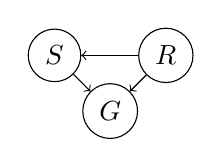
\begin{tikzpicture}[main/.style = {draw, circle}]  
    \node[main] (1) {$S$}; 
    \node[main] (2) [below right of=1] {$G$}; 
    \node[main] (3) [above right of=2] {$R$};
    \draw[->] (1) -- (2);
    \draw[->] (3) -- (1);
    \draw[->] (3) -- (2);
\end{tikzpicture} 
where R is father from G and S, S is parent from G, and the equation bellow is the respective bayesian probability
\begin{equation}
    P(S, R, G) = P(G|S, R)P(S|R)P(R)    
\end{equation}

\section{Class 5}
\subsection{Univariate Normal Distribution}
\begin{equation}
	\mathcal{N}(x|\mu, \sigma^2) = \frac{1}{\sqrt{2\pi\sigma^2}} e^{-\frac{(x - \mu)^2}{2\sigma^2}}    
\end{equation}
	
\subsection{Multivariate Normal Distribution}
\begin{equation}
    \mathcal{N}(x|\mu, \Sigma^2) = \frac{1}{\sqrt{2\pi\Sigma^2}} e^{-\frac{1}{2}(x - \mu)^T\Sigma^-1(x - \mu)}    
\end{equation}
		
\subsection{Linear Regression}
\begin{equation}
    L(w) = \sum_{i=1}^{N} (w^T x_i - y_i)^2 = ||w^T X - y|| \rightarrow \min_w
\end{equation}
\begin{equation}
    \hat{w} = arg \min_{w} L(w) 
\end{equation}
where $L$ is the loss from the bayesian net, $w$ are the weights and $X$ are the data, both are parents of $y$ (target)
\begin{equation}
    P(w, y|X) = P(y|X, w)P(w)
\end{equation}
\begin{equation}
    P(y|w, X) = \mathcal{N}(y|w^TX, \sigma^2\mathcal{I})
\end{equation}
\begin{equation}
    P(w) = \mathcal{N}(w|0, \gamma^2\mathcal{I}) 
\end{equation}
\begin{equation}
    P(w| y, x) = \frac{P(y, w|X)}{P(y|X)} \rightarrow \max_w
\end{equation}
\begin{equation}
    P(y, w|x) = \frac{P(y|x, w)}{P(w)} \rightarrow \max_w
\end{equation}

\section{Class 6}
\subsection{Maximum a Posteriori} 
To learn a distribution
\begin{equation}
    \theta_{MP} = arg \max_\theta P(\theta|X) = arg \max_\theta \frac{P(\theta|X)P(\theta)}{P(X)} = arg \max_\theta P(\theta|X)P(\theta)    
\end{equation}	
We eliminate the denominator from the last equation, once time it don't have $\theta$
Problems: \begin{itemize}
    \item it is not variant to reparametrization. Ex learning about a gaussian will be not usefull in sigmoid(gaussian)
	\item strange "loss function"
	\item we do not have the posteriori of $\theta$
	\item can't compute credible intervals
\end{itemize}		
			

\section{Class 7}
\subsection{Conjugate Distribution} 
It is a way to avoid computing the evidence ($P(X)$), which is costly. In the Bayes Probability
\begin{equation}
    P(\theta|X) = \frac{P(X|\theta)P(\theta)}{P(X)}
\end{equation}
in the likelihood, $P(X|\theta)$ is fixed by the model, $P(X)$ is fixed by the data, and $P(\theta)$ is our own choice. The prior $P(\theta)$ is conjugate to the likelihood if the prior and the posterior $P(X|\theta)$ lie in the same family distributions. 

\Eg if the prior is $P(X|\theta) = \mathcal{N}(x|\mu, \sigma^2)$ and the posterior is $P(\theta) = \mathcal{N}(\theta|m, s^2)$, thus the conjugate of posterior $P(\theta|X)$ is $\mathcal{N}(\theta|a, b^2)$.
\begin{equation}
    P(\theta|X) = \frac{P(X|\theta)P(\theta)}{P(X)} = \frac{\mathcal{N}(x|\theta, 1) \mathcal{N}(\theta|0, 1)}{P(X)}
\end{equation}
\begin{equation}
    P(\theta|X) \propto e^{-\frac{1}{2}(X - \theta)^2} e^{-\frac{1}{2}\theta^2}
\end{equation}
\begin{equation}
    P(\theta|X) \propto e^{-(\theta - \frac{X}{2})^2}
\end{equation}
\begin{equation}
    P(\theta|X) = \mathcal{N}(\theta|\frac{X}{2}, \frac{X}{2})
\end{equation}

\section{Class 8}

\subsection{Gamma Distribution}
\begin{equation}
    \Gamma(\gamma|a, b) = \frac{b^a}{\Gamma(a)} \gamma^{a-1}e^{-b\gamma}
\end{equation}
where \begin{itemize}
    \item $\gamma, a, b > 0$
    \item $\Gamma(n) = (n - 1)!$
    \item the expectation, or mean, $\mathbb{E}[\gamma] = \frac{a}{b}$
    \item $Mode[\gamma] = \frac{a-1}{b}$
    \item $Var[\gamma] = \frac{a}{b^2}$
\end{itemize}

\subsection{Precision}
\begin{equation}
    \gamma = \frac{1}{\sigma^2}
\end{equation}

If we replace the variance in the Normal Distribution to the inverse of the Precision, we get
\begin{equation}
    \mathcal{N}(x|\mu, \gamma^{-1}) = \frac{\sqrt{\gamma}}{\sqrt{2\pi}} e^{-\gamma\frac{(x - \mu)^2}{2}}    
\end{equation}
thus, the conjugate prior in respect to the precision is
\begin{equation}
    \mathcal{N}(x|\mu, \gamma^{-1}) \propto \gamma^{\frac{1}{2}}e^{-b\gamma}
\end{equation}
\begin{equation}
    P(\gamma) \propto \gamma^{a-1}e^{-b\gamma}
\end{equation}
\begin{equation}
    P(\gamma|X) = \Gamma(\gamma|a, b)
\end{equation}
then, the prior is
\begin{equation}
    P(\gamma|X) = \Gamma(\gamma|a, b) \propto  \gamma^{a-1}e^{-b\gamma}
\end{equation}
the posterior is
\begin{equation}
    P(\gamma|X) \propto P(X|\gamma)P(\gamma)
\end{equation}
dropping out all the constants, we have
\begin{equation}
    P(\gamma|X) \propto \left(\gamma^{\frac{1}{2}}e^{-\gamma \frac{(X - \theta)^2}{2}} \right) \left(\gamma^{a-1} e^{-b\gamma} \right)
\end{equation}
re-arranging the terms, we get
\begin{equation}
    P(\gamma|X) \propto \gamma^{\frac{1}{2} + a - 1}e^{-\gamma \frac{(X - \theta)^2}{2}} e^{-\gamma(b + \frac{(X - \mu)^2}{2})} 
\end{equation}
finally
\begin{equation}
    P(\gamma|X) = \Gamma(a + \frac{1}{2}, b + \frac{(X - \mu)^2}{2})
\end{equation}

\section{Class 9}
\subsection{Beta Distribution}
\begin{equation}
    \beta(X|a, b) = \frac{1}{\beta(a, b)}X^{a-1}(1 - X)^{b - 1}
\end{equation}
where:\begin{itemize}
    \item $X \in [0, 1]$
    \item $a, b > 0$
    \item \begin{equation}
        \beta(a, b) = \frac{\Gamma(a+b)}{\Gamma(a)\Gamma(b)}
    \end{equation}
    \item \begin{equation}
        \mathbb{E}[X] = \frac{a}{a+b}
    \end{equation}
    \item \begin{equation}
        Mode[X] = \frac{a-1}{a+b-2}
    \end{equation}
    \item \begin{equation}
        Var[X] = \frac{ab}{(a+b)^2(a+b-1)}
    \end{equation}
\end{itemize} 
\Eg to model a distribution with mean $0.8$ and standard deviation of $0.1$, thus $\mathbb{E}[X] = 0.8$ and $Var[X] = 0.1^2$. Consequently, a Beta distribution with $a = 12$ and $b = 3$ model it.

\subsection{Bernoulli Distribution}
The Beta distribution is the conjugate of the Bernoulli likelihood. \Eg a Bernoulli likelihood from a dataset
\begin{equation}
    P(X|\theta) = \theta^{N_1}(1-\theta)^{N_0}
\end{equation}
where $N_1$ is the number of ones in $X$ and $N_0$ the number of zeros. Thus, the Beta distribution is
\begin{equation}
    P(\theta) = \beta(\theta|a, b) \propto \theta^{a-1}(1-\theta)^{b-1}
\end{equation}
Multiplying the likelihood by the prior
\begin{equation}
    P(\theta|X) \propto P(X|\theta)P(\theta)
\end{equation}
using the before, but replacing the terms by the equivalent equations above, we have
\begin{equation}
    P(\theta|X) \propto \theta^{N_1}(1-\theta)^{N_0} \beta(\theta|a, b) \propto \theta^{a-1}(1-\theta)^{b-1}
\end{equation}
and rearranging the terms, we have
\begin{equation}
    P(\theta|X) \propto \theta^{N_1 + a - 1}(1 - \theta)^{N_0 + b - 1}
\end{equation}
and finally, recognizing the equation before as a Beta distribution, we have
\begin{equation}
    P(\theta|X) = \beta(N_1 + a, N_0 + b)
\end{equation}

\subsection{Posteriors}
\begin{itemize}
    \item Pros \begin{itemize}
        \item Exact posterior
        \item Easy for on-line learning. \Eg $P(\theta|X) = \beta(N_1 + a, N_2 + b)$
    \end{itemize}
    
    \item Cons \begin{itemize}
        \item In some cases, the conjugate prior may be inadequate
    \end{itemize}
\end{itemize}

\section{Class 10}
\subsection{Latent Variable} 
It is a hidden variable that you never observe. \Eg creating a dataset of a job interview, measuring the GPA, IQ, School degree, and Phone, from a first stage of the interview, and a last attribute Onsite performance, from the second interview. Traditional ML models will suffer with the missing data. Even more, probably there are some correlation between the variables, and ponder each combination will increase the number of attributes. Thus, we can link all these attributes with a latent variable, called in this example as Intelligence. We can model the problem as:
\begin{equation}
    P(X_1, X_2, X_3, X_4, X_5) = \sum_{i=1}^N P(X_1, X_2, X_3, X_4, X_5|I)P(I)
\end{equation}
where I is the latent variable. We can also simplify the problem with
\begin{equation}
    P(X_1, X_2, X_3, X_4, X_5) = \sum_{i=1}^N P(X_1|I)P(X_2|I)P(X_3|I)P(X_4|I)P(X_5|I)P(I)
\end{equation}
which breaks the table in 5 fewer tables, reduce the model complexity and improves the flexibility of the model.


\section{Class 12}
\subsection{Gaussian Mixture Model (GMM)}
It is a model of soft clustering with $N$ gaussian's can be described as
\begin{equation}
    P(X|\theta) = \pi_1\mathcal{N}(\mu_1, \Sigma_1) + \pi_2\mathcal{N}(\mu_2, \Sigma_2) + ... + \pi_N\mathcal{N}(\mu_N, \Sigma_N)
\end{equation}
where the $\theta$ weight matrix is 
\begin{equation}
    \theta = \{\pi_1, \pi_2, ..., \pi_N, \mu_1, \mu_2, ..., \mu_N, \Sigma_1, \Sigma_2, ..., \Sigma_N\}
\end{equation}
To goal of the train is
\begin{equation}
    \max_\theta P(X|\theta) = \prod_{i=1}^N P(X_1|\theta) = \prod_{i=1}^N \left( pi_1\mathcal{N}(\mu_1, \Sigma_1) + ... \right)
\end{equation}
By definition, the covariance matrix $\Sigma_k \succ 0$, once time we need to compute $\Sigma^{-1}$. Otherwise, we will have divisions by zero.

\section{Class 13}
Assuming that our data points $X$ was generated by a latent variable $t$. Thus, the probability of a point to belongs to the class $c$ given the parameters $\theta$ is
\begin{equation}
    P(t = c|\theta) = \pi_c
\end{equation}
and 
\begin{equation}
    P(X|t = c, \theta) = \mathcal{N}(X, \mu_c, \Sigma_c)
\end{equation}
Marginalizing the latent variable, we have
\begin{equation}
    P(X|\theta) = \sum_{c=1}^N P(X|t = c, \theta)P(t = c|\theta)
\end{equation}
which is the summation of the likelihood times the prior, and is exactly the same as the first equation, but ignoring the latent variable.

Training a GMM, if we have hard-labels of the points, it is a easy problem: we just need to compute the mean and standard deviation of each cluster. In the opposite side, if we have the parameters (consequently the gaussians), thus we can estimate the source ($P(t = 1|X, \theta) = \frac{P(X|t = 1, \theta)P(t = 1|\theta)}{Z}$), which is the joint probability (the likelihood times the prior). The problem of train a GMM is a Chicken and Egg problem:
\begin{itemize}
    \item Need gaussian parameters ($\theta$) to estimate the source (soft-labels)
    \item Need sources to estimate the gaussian parameters
\end{itemize}

\section{Class 14}
\subsection{EM GMM}
\begin{enumerate}
    \item Start with $N$ randomly placed gaussians parameters $\theta$
    \item Until convergence: \begin{enumerate}
        \item For each point $X_i$, compute $P(t = c|X_i, \theta)$
        \item Update gaussian parameters $\theta$ to fit points assigned to them
    \end{enumerate}
\end{enumerate}

\begin{itemize}
    \item EM can train GMM faster than Stochastic Gradient Descent
    \item EM suffers from local maxima (the exact solution is NP-Hard)
\end{itemize}

\section{Class 15}
\subsection{Concavity}
A function is concave if its second derivative is negative, or, if 
\begin{equation}
    f(\alpha a + (1 - \alpha)b) \geq \alpha f(a) + (1 - \alpha)f(b)
\end{equation}
where $0 \leq \alpha \leq 1$. The Figure \ref{fig:inequality} shows an \eg
\begin{figure}[!t]
    \centering
    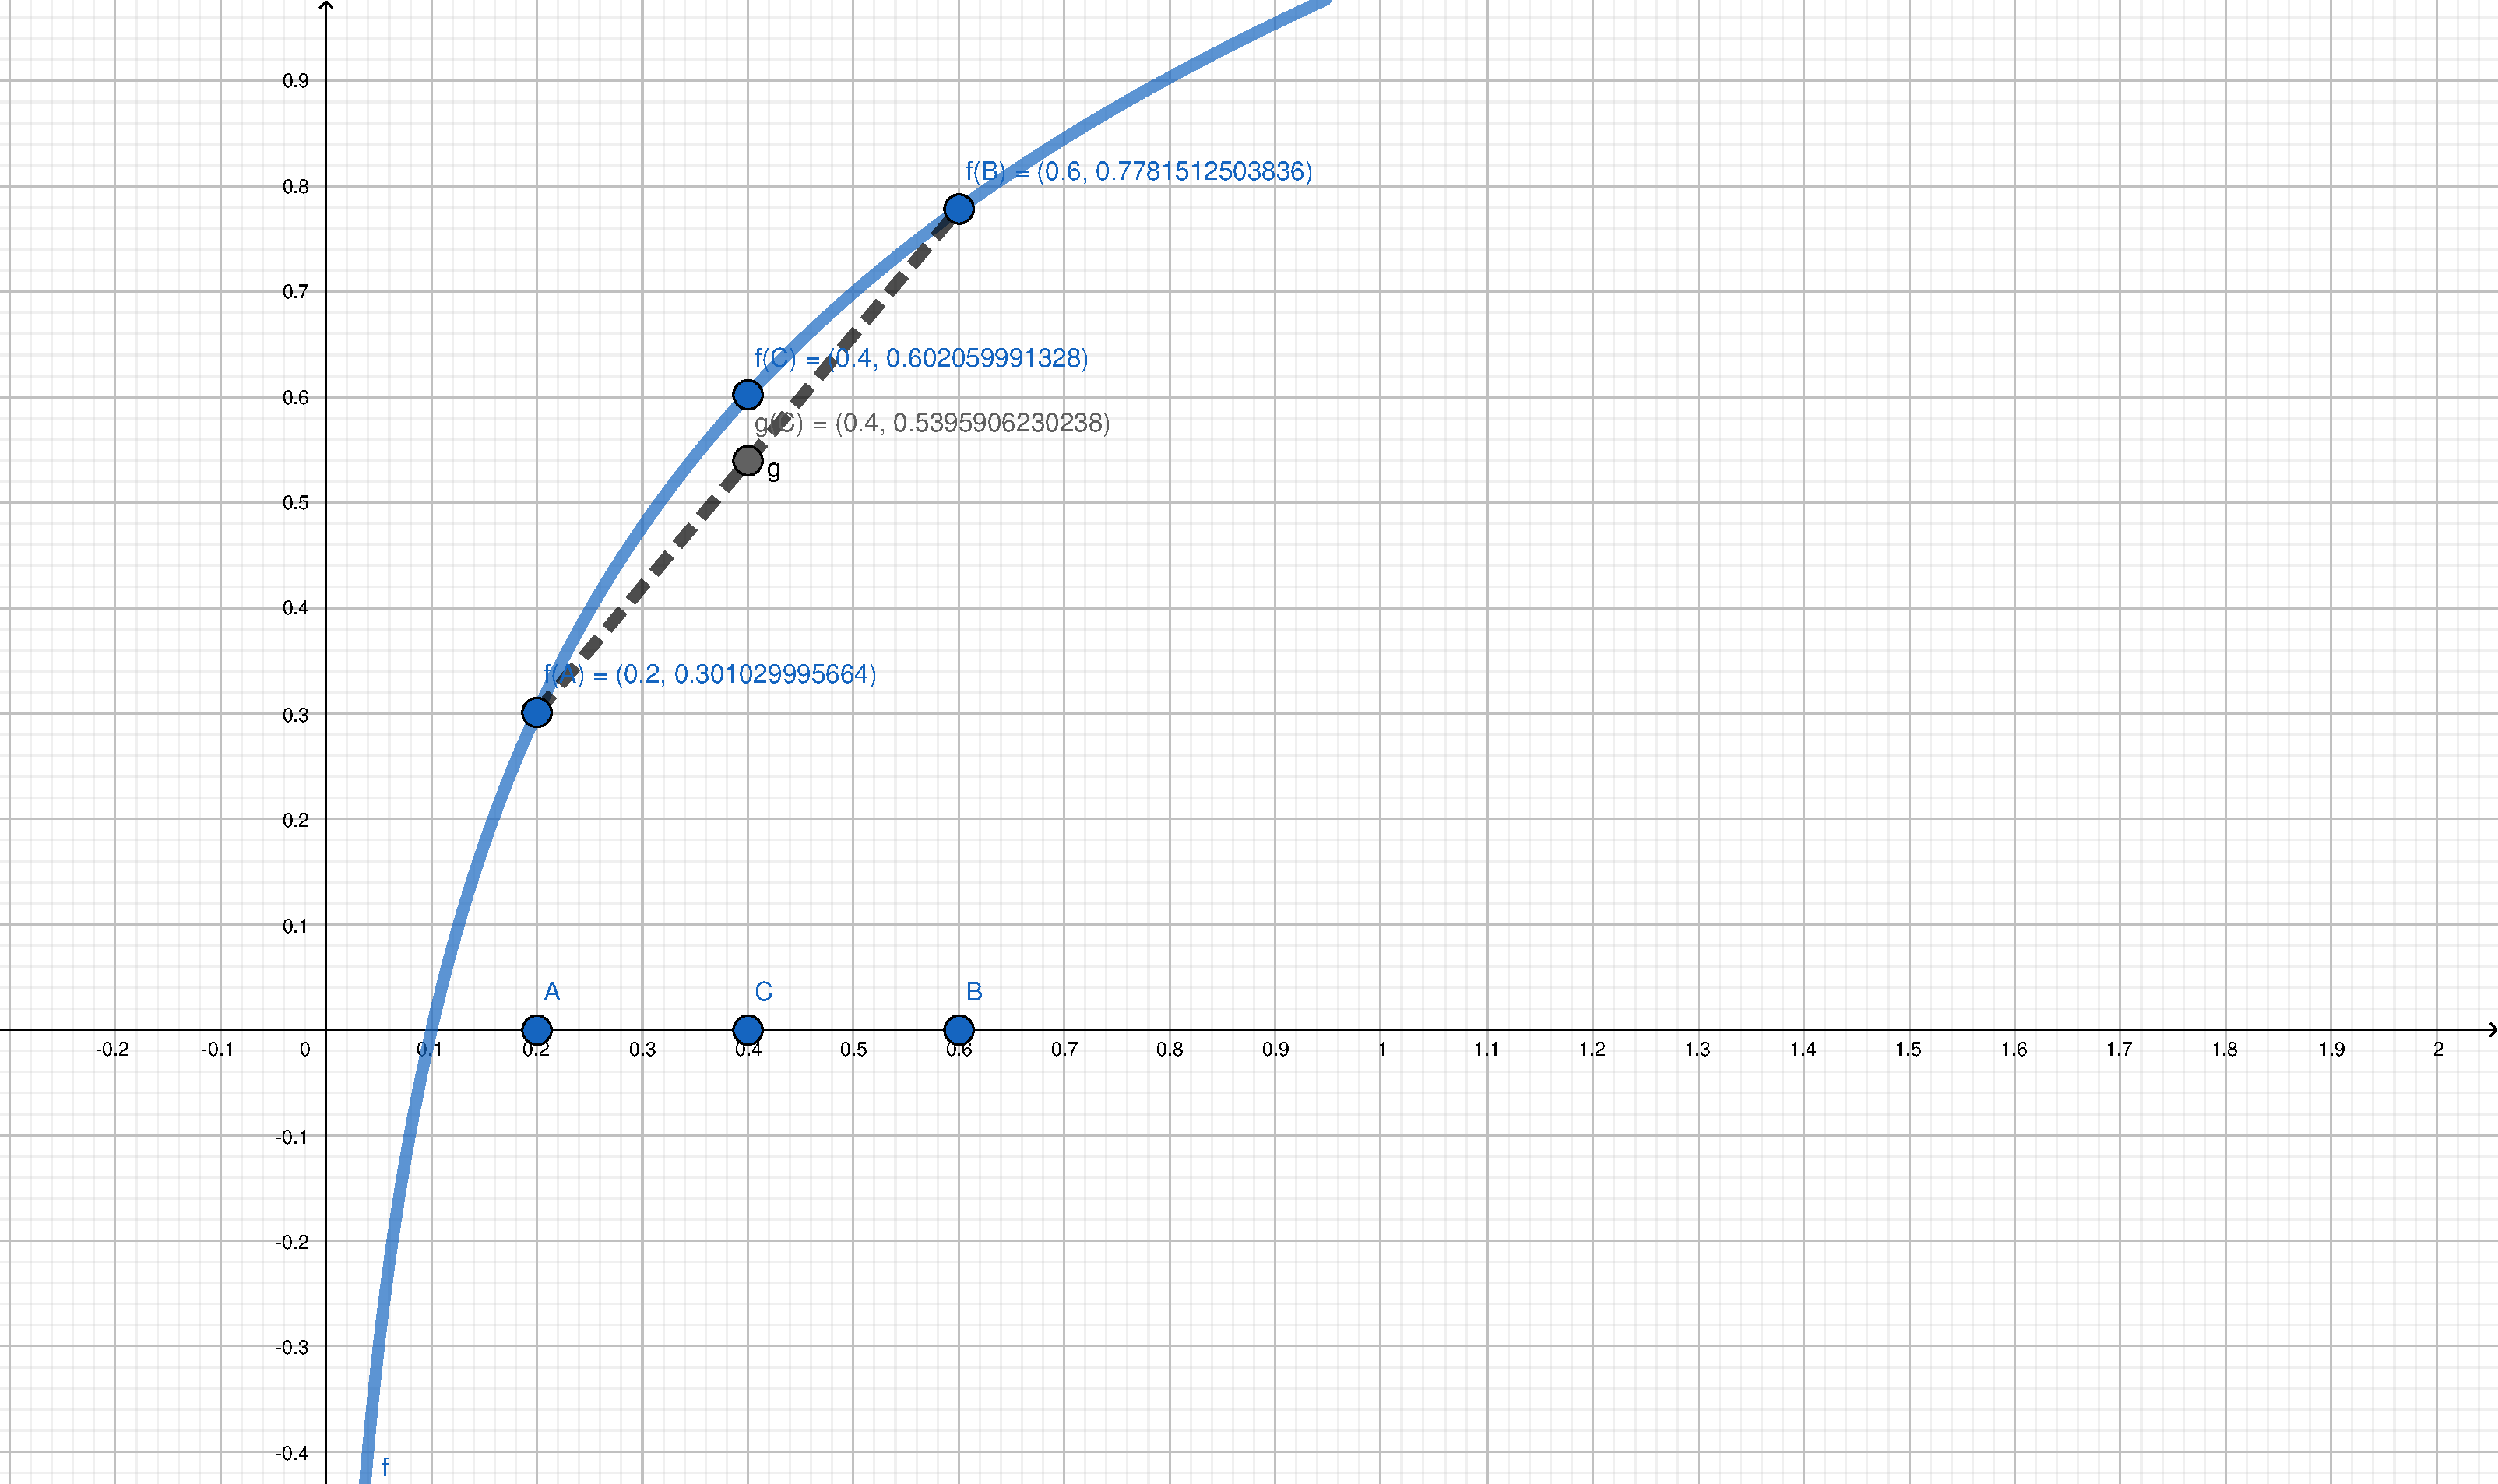
\includegraphics[width=\textwidth]{geogebra.pdf}
    \caption{Showing the inequality from the equation. The equation from the right inequality side, which generates the straight segment, we call as G(x).}
    \label{fig:inequality}
\end{figure}

\subsection{Jensen's inequality} 
Generalizing the concavity for any point, we have 
\begin{equation}
    f(\mathbb{E}_{p(t)t}) \geq \mathbb{E}_{p(t)}f(t)
\end{equation}

\subsection{Kullback-Leibler Divergence} 
It is a way to measure the difference between two probabilistic functions.
\begin{equation}
    \mathcal{K}\mathcal{L}(p || q) = \int q(x) \log \frac{q(x)}{p(x)} dx
\end{equation}
Properties: \begin{enumerate}
    \item \begin{equation}
        \mathcal{K}\mathcal{L}(p || q) \neq \mathcal{K}\mathcal{L}(q || p)
    \end{equation}
    \item \begin{equation}
        \mathcal{K}\mathcal{L}(q || q) = 0
    \end{equation}
    \item \begin{equation}
        \mathcal{K}\mathcal{L}(p || q) > 1
    \end{equation}
\textcolor{red}{Proof}
\begin{equation}
    - \mathcal{K}\mathcal{L}(p || q) = \mathbb{E}_q \left(-\log \frac{q}{p} \right) = \mathbb{E}_q \left(\log \frac{p}{q} \right)
\end{equation}
\begin{equation}
    \leq \log \left(\mathbb{E}_q \frac{p}{q} \right) = \log \int q(x) \frac{p(x)}{q(x)}dx = 0
\end{equation}
\end{enumerate}

\end{document}